\documentclass[12pt,a4paper]{article}
\usepackage[utf8]{inputenc}
\usepackage[T2A]{fontenc}
\usepackage[ukrainian]{babel}
\usepackage{fancyvrb}

\usepackage{amsmath} % у преамбулі
\usepackage{hyperref} % <-- Обов’язково підключіть цей пакет
\usepackage{caption}
\captionsetup[table]{name=Таблиця}  % замість "Табл." буде "Таблиця"

\usepackage{xcolor}

\renewcommand{\thetable}{№\arabic{table}}

\usepackage{graphicx} % <-- Для роботи з \includegraphics
\usepackage{geometry}
\geometry{
    left=2cm,
    right=2cm,
    top=2cm,
    bottom=2cm
}

\begin{document}

    \begin{titlepage}

        \thispagestyle{empty}
        \begin{center}
        \large
        Національний технічний університет України\\
        «Київський політехнічний інститут імені Ігоря Сікорського»\\[1em]
        Факультет інформатики та обчислювальної техніки\\
        Кафедра загальної фізики
        \end{center}

        \vfill

        \begin{center}
        \textbf{\LARGE Фізика}\\[2em]
        \textbf{\Large Лабораторна робота №ФПЕ-10}\\
        «Дослідження згасаючих коливань у коливальному контурі» 
        \end{center}

        \vfill

        \begin{flushright}
        Виконав: студент 1 курсу ФІОТ, гр. ІО-41\\
        \textit{Давидчук А. М.}\\
        Залікова книжка № 4106\\[1em]
        Перевірив: \textit{Колган В.\,В.}
        \end{flushright}

        \vfill

        \begin{center}
        Київ -- 2025
        \end{center}

    \end{titlepage}

    \setlength{\parindent}{0pt}

    % main document

    \textbf{\underline{Тема:}} «Дослідження згасаючих коливань у коливальному контурі».

    \vspace{1em} % вручну задаєте відступ

    \textbf{\underline{Мета:}} визначення параметрів та характеристик реального коливального контуру.

    \vspace{1em} % вручну задаєте відступ

    \textbf{\underline{Прилади та устаткування:}} Блок-схема експериментальної установки (рис. 3.1): ГЗ-111 --- генератор звукових сигналів ГЗ-111; С1-76 --- осцилограф С1-76;
    ФПЭ-10/11 --- касета з контуром ФПЕ-10/11; ПІ-ФПЭ-09 --- перетворювач імпульсів; Дж --- джерело живлення; МО --- магазин опорів.

    \begin{figure}[h!]

        \setcounter{figure}{0}                  % скидаємо лічильник фігур
        \renewcommand{\thefigure}{3.\arabic{figure}} % робимо "3.1", "3.2" і т.д.

        \centering
        % Підставляєте потрібний шлях та розмір зображення:
        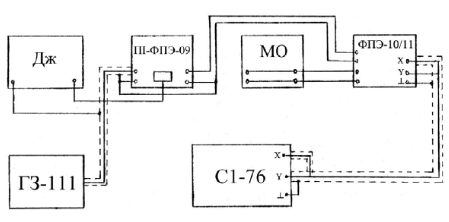
\includegraphics[width=0.5\textwidth]{3.1.png}
        % Підпис (зазвичай під малюнком):
        \caption{Загальна схема досліду}
        % Мітка для посилань у тексті (\ref{fig:...})
        \label{fig1:schema}
    \end{figure}

    %%%%%%%%%%%%%%%%%%%%%%%%%%%%%%%%%%%Теоретичні відомості%%%%%%%%%%%%%%%%%%%%%%%%%%%%%%%%%%%

    \begin{center}
        \textbf{\Large Теоретичні відомості}
    \end{center}

    \vspace{1em} % вручну задаєте відступ

    \setlength{\parindent}{1.5em}

    Реальний коливальний контур складається з послідовно з’єднаних конденсатора $C$, котушки індуктивності $L$
    і резистора $R$. Якщо зарядити конденсатор від батареї Б до напруги $U$ (рис. 3.2), а потім від’єднати батарею
    за допомогою ключа $K$, то конденсатор почне розряджатися через котушку і у контурі виникнуть електромагнітні коливання.

    \begin{figure}[h!]

        \renewcommand{\thefigure}{3.\arabic{figure}} % робимо "3.1", "3.2" і т.д.

        \centering
        % Підставляєте потрібний шлях та розмір зображення:
        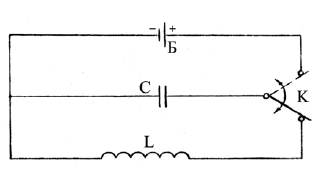
\includegraphics[width=0.5\textwidth]{3.2.png}
        % Підпис (зазвичай під малюнком):
        \caption{Загальна схема досліду}
        % Мітка для посилань у тексті (\ref{fig:...})
        \label{fig2:schema}

    \end{figure}

    Спочатку розглянемо випадок, коли опір контуру $R$ = 0.

    Після замикання контуру в ньому виникне розрядний струм $I$, який не відразу набуває максимального значення.
    Плавна зміна сили струму в колі зумовлена появою в котушці ЕРС самоіндукції, яка за правилом Ленца перешкоджає зміні струму,
    тобто гальмує розряд конденсатора. Як тільки заряд конденсатора стане рівним нулю, сила струму в контурі досягне максимуму.
    З цього моменту сила струму в колі починає зменшуватися, не змінюючи свого напрямку.
    В цьому випадку ЕРС самоіндукції підтримує струм, який викликав її появу.
    Ця ж ЕРС призводить до перезаряджання конденсатора, після чого процес повторюється, однак з іншим напрямом струму.
    Надалі ці процеси повторюються, тобто виникають коливання.

    Час, протягом якого в коливальному контурі відбувається один повний цикл змін і контур повертається в початковий стан, називають періодом електричного коливання.

    Якщо активний опір в контурі дорівнює 0, то коливання в контурі можуть продовжуватися нескінченно довго.
    Такі коливання, які відбуваються внаслідок процесів у самому коливальному контурі без зовнішніх впливів і втрат енергії,
    називають власними електричними коливаннями. Вони є незагасаючими.

    У початковий момент, коли конденсатор був заряджений, у ньому була накопичена енергія

    \begin{center}
        $\displaystyle W_e = \frac{CU^2}{2}.$
    \end{center}

    Під час розрядки енергія електричного поля конденсатора перетворюється в енергію магнітного поля котушки і,
    коли конденсатор повністю розряджений, енергія магнітного поля досягає максимального значення:

    \begin{center}
        $\displaystyle W_m = \frac{LI_0^2}{2}$,
    \end{center}

    де $I_0$ --- амплітуда сили струму в контурі. Під час перезаряджання конденсатора енергія магнітного поля знову перетворюється на енергію електричного поля.
    За умови $R$ = 0 у контурі відбуваються незагасаючі електромагнітні коливання.

    Усі без винятку провідники за звичайних умов мають відмінний від нуля опір, тому частина енергії при
    коливаннях витрачається на їх нагрівання, тобто перетворюється на теплову і втрачається.
    В наслідок цього амплітуда електромагнітних коливань в контурі зменшується
    відбувається загасання коливань (рис. 3.3).

    \begin{figure}[h!]

        \renewcommand{\thefigure}{3.\arabic{figure}} % робимо "3.1", "3.2" і т.д.

        \centering
        % Підставляєте потрібний шлях та розмір зображення:
        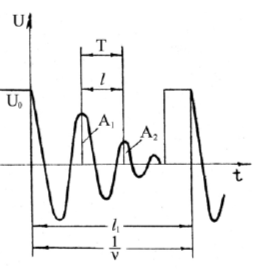
\includegraphics[width=0.3\textwidth]{3.3.png}
        % Підпис (зазвичай під малюнком):
        \caption{Графік згасаючих коливань}
        % Мітка для посилань у тексті (\ref{fig:...})
        \label{fig3:schema}

    \end{figure}

    При достатньо великому опорі контуру або малій індуктивності коливання у ньому взагалі не виникають,
    а відбувається так званий аперіодичний розряд конденсатора.

    Заряд конденсатора і сила струму у котушці коливального контуру постійно змінюються
    за значенням і напрямом. Вважатимемо, що в момент часу $t$ заряд на обкладинках
    конденсатора $q$, напруга на ньому $\displaystyle U_C = \frac{q}{C}$, а сила струму у колі
    змінюється зі швидкістю $\displaystyle \frac{dI}{dt}$. У котушці індуктивності виникає ЕРС самоіндукції

    \begin{equation}
        \mathcal{E}_L = -L\frac{dI}{dt}.
        \tag{3.1}
    \end{equation}

    Відповідно до другого правила Кірхгофа для коливального контуру, опір якого дорівнює нулю, можна записати

    \begin{equation}
        U + \mathcal{E}_L = IR,
        \tag{3.2}
    \end{equation}

    де

    \begin{equation}
        I = -\frac{dq}{dt}.
        \tag{3.3}
    \end{equation}

    (струм тече в додатному напрямку при зменшенні заряду конденсатора).

    Оскільки $q = CU$, то з урахуванням (3.1) та (3.2) отримаємо:

    \begin{center}
        $\displaystyle I = -C \frac{dU}{dt}$,
    \end{center}

    \begin{center}
        $\displaystyle \mathcal{E}_L = LC \frac{d^2U}{dt^2}$.
    \end{center}

    Підставивши останній вираз в (3.2), матимемо:

    \begin{equation}
        \frac{d^2U}{dt^2} + \frac{R}{L} \frac{dU}{dt} + \frac{U}{LC} = 0.
        \tag{3.4}
    \end{equation}

    Як відомо, диференціальне рівняння (3.4) є рівнянням загасаючих електричних коливань.
    Розв’язком цього рівняння є функція

    \begin{equation}
        U = U_0e^{-\beta t} \cos(\omega t + \alpha).
        \tag{3.5}
    \end{equation}

    де $\beta$ --- коефіцієнт загасання,

    \begin{equation}
        \beta = \frac{R}{2L},
        \tag{3.6}
    \end{equation}

    де $\omega$ --- циклічна частота загасаючих коливань,

    \begin{equation}
        \omega = \sqrt{\frac{1}{LC} - \left( \frac{R}{2L}\right)^2}.
        \tag{3.7а}
    \end{equation}

    При цьому

    \begin{equation}
        \omega = \frac{2\pi}{T} \text{  та  } T = \frac{2\pi}{\sqrt{\dfrac{1}{LC} - \left( \dfrac{R}{2L}\right)^2}}.
        \tag{3.7б}
    \end{equation}

    Якщо (3.2) записати у вигляді

    \begin{center}
        $\displaystyle \frac{q}{C} + IR = -\frac{dI}{dt}$
    \end{center}

    та взяти похідну за часом, то отримаємо рівняння подібне до рівняння (3.4):

    \begin{center}
        $\displaystyle \frac{d^2I}{dt^2} + \frac{R}{L} \frac{dI}{dt} + \frac{I}{LC} = 0$.
    \end{center}

    Отже, сила струму $I$ в контурі також здійснює загасаючі коливання (щоправда, початкова фаза цих коливань буде іншою),
    для яких значення $\beta$ й $\omega$ визначаються формулами (3.6), (3.7а) та (3.7б).

    З (3.7а) та (3.7б) видно, що в коливальному контурі можливі загасаючі коливання лише у випадку,
    якщо $\displaystyle \frac{1}{LC} > \left( \frac{R}{2L}\right)^2$ (частота та період є дійсними величинами)
    або $\displaystyle R < 2\sqrt{\frac{L}{C}}$, то частота і період – уявні величини, коливань немає і відбувається
    аперіодичний розряд конденсатора.

    Опір

    \begin{equation}
        R_{cr} = 2\sqrt{\frac{L}{C}}
        \tag{3.8}
    \end{equation}

    називають критичним.

    Щоб характеризувати загасаючі коливання, окрім коефіцієнта загасання $\beta$,
    використовується ще логарифмічний декремент (лат. dekrement --- зменшення) загасання.

    Логарифмічним декрементом загасання називається натуральний логарифм
    відношення значень напруги, розділених інтервалом часу,
    який дорівнює періоду коливань $T$,

    \begin{equation}
        \lambda = \ln \frac{A_1}{A_2} = \ln \frac{A(t)}{A(t+T)},
        \tag{3.9}
    \end{equation}

    або

    \begin{center}
        $\displaystyle \lambda \approx 2,3\cdot \lg \frac{A_1}{A_2}$.
    \end{center}

    Підставивши в (3.9) значення $A(t) = U_0e^{-\beta t}$ та $A(t+T) = U_0e^{-\beta (t+T)}$, отримаємо

    \begin{equation}
        \lambda = \beta T,
        \tag{3.10}
    \end{equation}

    або згідно (3.6)

    \begin{equation}
        \lambda = \frac{R}{2L}T.
        \tag{3.10а}
    \end{equation}

    У деяких випадках зручно вивчати коливний процес у системі координат $I$ та $U$,
    тобто відкладати на осі абсцис значення сили струму в контурі,
    а на осі ординат -- напругу на конденсаторі у той же момент часу.
    Площина $IU$ має назву площини станів, або фазової площини, а крива,
    яка зображає залежність напруги від струму, називається фазовою кривою (див. рис. 3.4).

    \begin{figure}[h!]

        \renewcommand{\thefigure}{3.\arabic{figure}} % робимо "3.1", "3.2" і т.д.

        \centering
        % Підставляєте потрібний шлях та розмір зображення:
        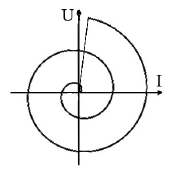
\includegraphics[width=0.3\textwidth]{3.4.png}
        % Підпис (зазвичай під малюнком):
        \caption{Фазова крива}
        % Мітка для посилань у тексті (\ref{fig:...})
        \label{fig4:schema}

    \end{figure}

    Знайдемо фазову криву для контуру, опір якого $R = 0$. цьому випадку
    $\displaystyle \beta = \frac{R}{2L} = 0$ і тоді з (3.5), (3.7а) та (3.7б) отримуємо

    \begin{equation}
        \omega = \sqrt{\frac{1}{LC}},\text{ } T = 2\pi \sqrt{LC},
        \tag{3.11}
    \end{equation}

    \begin{equation}
        \left\{
        \begin{aligned}
            U &= U_0 \cos \omega t \\
            I &= -C \frac{dU}{dt} = U_0 \omega C \sin \omega t
        \end{aligned}
        \right.
        \tag{3.12}
    \end{equation}

    Рівняння (3.11), (3.12) описують незагасаючі коливання.
    Виключивши з них час $t$, отримаємо рівняння фазової кривої (рівняння еліпса):

    \begin{center}
        $\displaystyle \frac{U^2}{U_0^2} - \frac{I^2}{U_0^2 \omega^2 C^2} = 1$.
    \end{center}

    Еліпс можна отримати у результаті накладання двох взаємно перпендикулярних
    гармонічних коливань (3.12), із зсувом фаз у чверть періоду.

    У контурі, опір якого $R>0$, відбуваються загасаючі коливання напруги (3.5) та струму:
    \begin{center}
        $
        \left\{
        \begin{aligned}
            U &= U_0 e^{-\beta t} \cos \omega t \\
            I &= -C \frac{dU}{dt} = U_0C e^{-\beta t} (\beta \cos \omega t + \omega \sin \omega t)
        \end{aligned}
        \right.
        $
    \end{center}

    У цьому випадку амплітуди напруги та сили струму у контурі безперервно
    спадають і фазова крива буде незамкненою (рис.3.4).

    У даній роботі для отримання коливань у контурі використовується касета
    ФПЕ-10/11 з контуром, зображеним на рис. 3.5.

    \begin{figure}[h!]

        \renewcommand{\thefigure}{3.\arabic{figure}} % робимо "3.1", "3.2" і т.д.

        \centering
        % Підставляєте потрібний шлях та розмір зображення:
        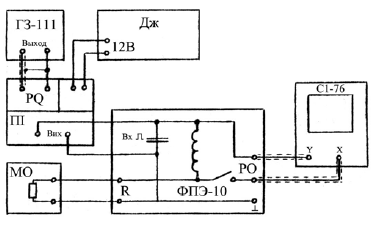
\includegraphics[width=0.5\textwidth]{3.5.png}
        % Підпис (зазвичай під малюнком):
        \caption{Схема експериментальної установки}
        % Мітка для посилань у тексті (\ref{fig:...})
        \label{fig5:schema}

    \end{figure}

    Загасаючі коливання, які відбуваються у контурі, спостерігаються на екрані
    осцилографа С1-76. Цикл зарядки та розрядки конденсатора продовжується
    протягом часу $T = \dfrac{1}{v}$, де $v$ – частота, яка задається звуковим
    генератором ГЗ-111. На екрані осцилографа йому відповідає відрізок $l_1$.
    Це дозволяє визначити період $T$ загасаючих коливань,
    якому на рис. 3.3 відповідає відрізок l. З пропорції $\dfrac{l}{T} = l_1v$ отримаємо

    \begin{equation}
        T = \frac{l}{l_1v}.
        \tag{3.14}
    \end{equation}

    %%%%%%%%%%%%%%%%%%%%%%%%%%%%%%%%%%%Теоретичні відомості%%%%%%%%%%%%%%%%%%%%%%%%%%%%%%%%%%%

    \newpage

    \begin{center}
        \textbf{\Large Практична частина}
    \end{center}

    \vspace{1em} % вручну задаєте відступ

    \setlength{\parindent}{0pt}

    \textbf{Порядок виконання завдання №1:}

    \vspace{1em} % вручну задаєте відступ

    \setlength{\parindent}{1.5em}

    1. Включив лабораторний стенд і переконався, що він готовий до роботи (загорілася лампочка «Сеть»).

    2. Запустив генератор сигналів ГЗ-111 та виставив частоту $\nu = 250$ Гц.

    3. Включив джерело живлення та активував перетворювач імпульсів ПІ-ФПЕ-09, вибравши відповідні налаштування (клавіша «П» і «Скважность грубо»).

    4. На магазині опорів послідовно встановлював значення $R_m = $ 100, 200, 300, 400, 500, 600 Ом.

    5. За допомогою осцилографа С1-76 отримував стабільну картину загасаючих коливань.

    6. Виміряв довжини відрізків $l$ і $l_1$ на екрані осцилографа та розрахував період коливань $T$ за формулою (3.14).

    7. Виміряв значення амплітуд коливань ($A_1$, $A_2$, $A_3$) та розрахував логарифмічний декремент $\lambda$ за формулою (3.9), а також коефіцієнт загасання $\beta$ за формулою (3.10) для кожного зі значень $R_m$. Всі результати заніс у таблицю №1.

    8. Побудував графік залежності $\lambda$ від опору магазину опорів $R_m$, визначивши внутрішній опір котушки $r_k$ за допомогою екстраполяції графіка $\lambda(R_m)$ до 0. Відовідно, обчислишви значення $r_k$, я обчислив значення повного
    опору $R$ для кожного значення опору $R_m$: $R = R_m + r_k$.

    9. Розрахував середні значення індуктивності $L$ з формули (3.10а) і ємності $C$ контуру з формули (3.11) періоду для мого досліду. Тобто

    \begin{center}
        $\displaystyle L = \frac{R}{2\lambda} T$ \text{  та  } $\displaystyle C = \left( \frac{T}{2\pi} \right)^2 \cdot \frac{1}{L}$.
    \end{center}

    10. Визначив критичний опір $R_{cr}$ за формулою (3.15), за якого спостерігається аперіодичний розряд конденсатора, і перевірив відповідність цього значення розрахунковим співвідношенням.

    \begin{equation}
        R_{cr} = 2 \sqrt{\frac{L}{C}}.
        \tag{3.15}
    \end{equation}

    \vspace{1em} % вручну задаєте відступ

    \setlength{\parindent}{0pt}

    \textbf{Порядок виконання завдання №2:}

    \vspace{1em} % вручну задаєте відступ

    \setlength{\parindent}{1.5em}

    1. Перевів осцилограф у режим фазової діаграми.
    
    2. Встановлював фазові криві в центр екрана та вимірював значення вертикальної напруги $U$ та горизонтальної $U$ екрана осцилографа з кроком в одни період.

    3. За формулою (3.9) обчислював логарифмічний декремент $\lambda$ як за вертикальною напругою (вже обчислені дані в таблиці №1), так і за силою струму, яку можна знайти з відношення $U = IR_m$.

    4. Результати всіх вимірювань заносив до таблиці №2.

    5. Оцінив похибку вимірювань логарифмічного декременту для $U$ та $I$ за формулою

    \begin{center}
        $\displaystyle \Delta \lambda_X = \sqrt{\frac{\Delta X_1^2}{X_1} + \frac{\Delta X_2^2}{X_2}}, \quad X = 
        \begin{cases}
        U\\
        I
        \end{cases}$
    \end{center}

    \vspace{1em} % вручну задаєте відступ
    \setlength{\parindent}{0pt}

    \textbf{Всі вимірювання проводив у симуляторі лабораторної роботи ФПЕ-10 (FPE10)!}

    \newpage

    \textbf{\large Завдання №1:}

    \vspace{1em} % вручну задаєте відступ

    Під час вимірювань величин $l$ та $l_1$, я отримав такі значення:

    \vspace{1em} % вручну задаєте відступ

    $l = 4 \cdot 10^{-3}$ с, $l_1 = 0,4 \cdot 10^{-3}$ с.

    \vspace{1em} % вручну задаєте відступ

    Звідси $T$ = $\displaystyle \frac{l}{l_1 \nu} = \frac{0,4 \cdot 10^{-3}}{4 \cdot 10^{-3} \cdot 250} = \frac{0,4 \cdot 10^{-3}}{1} = 0,4 \cdot 10^{-3}$ с.

    \vspace{1em} % вручну задаєте відступ
    \setlength{\parindent}{1.5em}

    Далі змінюватиму $R_m$, вимірюватиму величини $A_1$, $A_2$, $A_3$ та за наявних даних, обчислю всі значення таблиці за допомогою Python коду (\hyperlink{listing1}{Лістинг 3.1}).
    Значення $r_k$ я знайду, побудувавши графік $\lambda(R_m)$ та знайшовши точку перетину з віссю абсцис (див. рис. 3.6).

    \begin{table}[h!]
        \centering
        \renewcommand{\arraystretch}{1.2} % відстань між рядками
        \begin{tabular}{|c|c|c|c|c|c|c|c|c|c|}
            \hline
            $R_m$, Ом & $A_1$, В & $A_2$, В & $A_3$, В & $\lambda$ & $\beta$, c$^{-1}$ & $L$, Гн & $C$, мкФ & $r_k$, Ом & $R$, Ом \\[3pt]
            \hline
            100 & 5,4547 & 4,5516 & 3,8292 & 0,2359 & 589,7 & 0,1382 & 0,0293 & 63,0058 & 163 \\[3pt]
            200 & 4,8768 & 3,6485 & 2,7093 & 0,3919 & 979,7 & 0,1342 & 0,0301 & & 263 \\[3pt]
            300 & 4,3710 & 2,8899 & 1,8785 & 0,5630 & 1408,0 & 0,1290 & 0,0314 & & 363 \\[3pt]
            400 & 3,9014 & 2,2758 & 1,3366 & 0,7141 & 1785,0 & 0,1297 & 0,0312 & & 463 \\[3pt]
            500 & 3,4679 & 1,8423 & 0,9392 & 0,8709 & 2177,0 & 0,1293 & 0,0313 & & 563 \\[3pt]
            600 & 3,0706 & 1,4450 & 0,6864 & 0,9988 & 2497,0 & 0,1328 & 0,0305 & & 663 \\[3pt]
            \hline
        \end{tabular}
        \caption{Результати розрахунку $\lambda$, $\beta$, $R$, $L$, $C$ коливального контуру.}
    \end{table}

    \begin{figure}[h!]

        \renewcommand{\thefigure}{3.\arabic{figure}} % робимо "3.1", "3.2" і т.д.

        \centering
        % Підставляєте потрібний шлях та розмір зображення:
        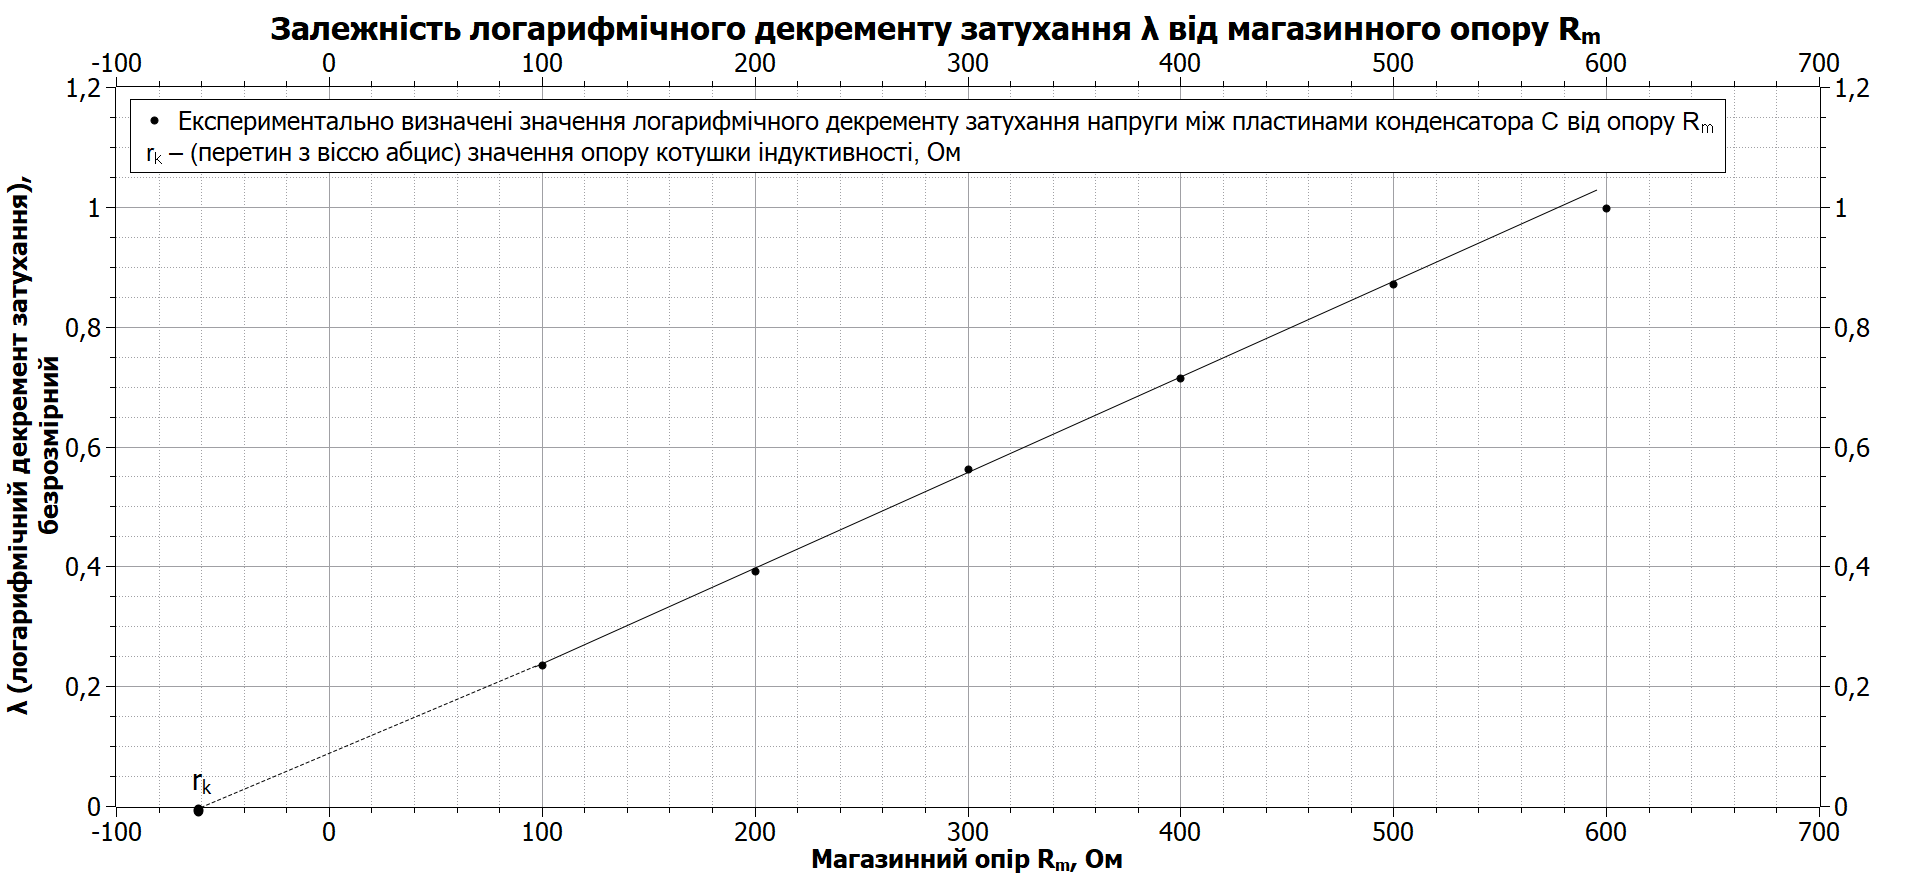
\includegraphics[width=1.00\textwidth]{graph.png}
        % Підпис (зазвичай під малюнком):
        \caption{Графік $\lambda(R_m)$}
        % Мітка для посилань у тексті (\ref{fig:...})
        \label{graph:schema}

    \end{figure}

    Також додатково було пораховано середнє значення індуктивності $L$, ємності $C$ контуру, як середнє арифметичне значення в таблиці №1 та відносно них
    $R_{cr}$ за формулою (3.15):

    \vspace{1em} % вручну задаєте відступ
    \setlength{\parindent}{0pt}

    ⟨$L$⟩ = 0,1322 Гн; ⟨$C$⟩ = 0,0307 мкФ;   $R_{cr}$ = 4088,5 Ом.

    \newpage

    Графік, що демонструє аперіодичне коливання при критичному опорі контуру $R_{cr}$:

    \begin{figure}[ht]
        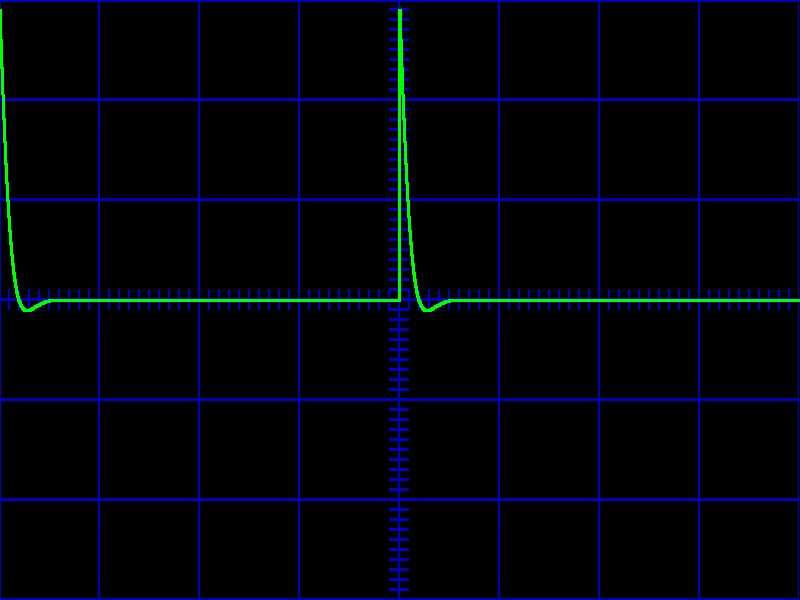
\includegraphics[width=0.9\textwidth]{aperiodic1.jpg}
    \end{figure}

    \vspace{1em}

    Результат виконання програми з \hyperlink{listing1}{Лістингу 3.1}:

    \begin{figure}[ht]
        \centering
        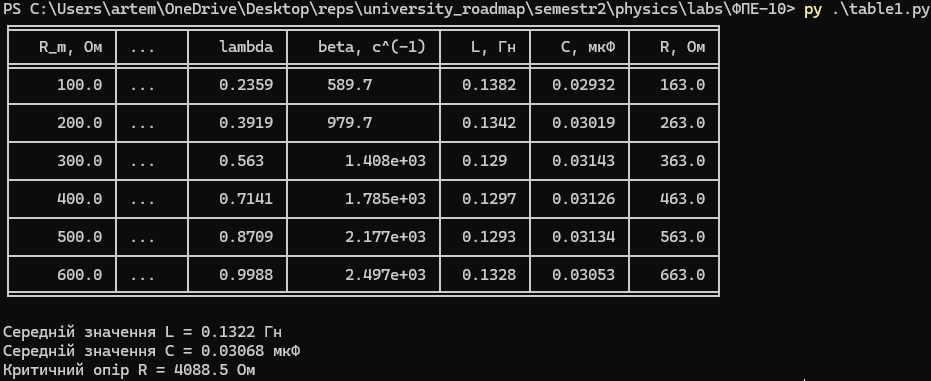
\includegraphics[width=1\textwidth]{table1.png}
    \end{figure}

    \vspace{1em} % вручну задаєте відступ

    \textbf{\large Обчислення похибок для завдання №1:}

    \vspace{1em} % вручну задаєте відступ
    \setlength{\parindent}{1.5em}

    В ході виконання завдання №1, використовувались такі величини: експериментально визначені значення (пряме вимірювання) $R_m$, $l$, $l_1$, $A_i$, де $i = \overline{1, 3}$ та $r_k$;
    теретично визначені значення (непрямі вимірювання) $T$, $\lambda$, $\beta$, $R$, $L$, $C$ та $R_{cr}$. Почнемо розгляд з експериментально визначених величин.

    Величини $R_m$ та $r_k$ які являються опорами, тобто теоретично їх можна розглядати, як опір 2 резисторів. Зазвичай, резистори,
    які використовуються в лабораторній роботі мають клас точності 5\%, тобто відносна похибка для резистора $R$ та $r_k \approx$ 5\% = 0,05. Абсолютну похибку
    вираховують шляхом множення номінального значення резистора на його відносну похибку. З резистором $r_k$ все дуже прозоро, так як цей резистор статичний, прийнамні, не враховується його зміна через зміну температури.
    І його абсолютна похибка буде $\Delta r_k = r_k \cdot 0,05 = 63,0058 \cdot 0,05 \approx 3,15$ Ом. Ось ситуація з опором $R_m$ складніша: ми використовували його із різними значеннями.
    В такому випадку, я знайду середнє арифметичне значення $R_m$ в діапазоні змін, тобто від 100 до 600, а потім отриманий результат помножу на відносну похибку 5\%.

    \vspace{1em} % вручну задаєте відступ
    \setlength{\parindent}{0pt}

    $\displaystyle \Delta R_m \approx \frac{R_{m_i}}{6} \cdot 0,05, i = \overline{1, 6} \approx \frac{100 + 200 + 300 + 400 + 500 + 600}{6} \cdot 0,05 = \frac{2100}{6} \cdot 0,05 = 17,5$ Ом.

    \setlength{\parindent}{1.5em}

    Щодо величин $l_1$ та $l$ --- вони були визначені за допомогою поділок на екрані осцилографа. Ціна однієї поділки в режимі залежності $U = f(t)$ на осі абцис $\Delta t$ = $10^{-3}$ с. Так як даних про похибку
    самого зображення на екрані осцилографа у нас немає, візьмемо середнє поширене значення в 3\%. Аболютну похибку для $l_1$ та $l$ можна обчислити за формулою

    \begin{center}
        $\displaystyle \Delta l = \sqrt{(\Delta T_k)^2 + (\Delta T_c)^2}$,
    \end{center}

    де $\Delta T_k$ --- похибка калібрування осцилографа, $\Delta T_k = T \cdot 0,03$, а $\Delta T_c$ --- похибка вимірювання, $\Delta T_c = \Delta t \cdot k$, де $k = 0,2$ --- похибка відліку для екрану осцилографа.
    Тут за $T$ ми приймаємо значення $l$ та $l_1$. Відносні похибки можна обчислити за формулою $\displaystyle \varepsilon = \frac{\Delta l}{l}$.

    Для $l$ матимемо:

    \vspace{1em} % вручну задаєте відступ

    $\displaystyle \Delta T_k = 0,4 \cdot 10^{-3} \cdot 0,03 = 12 \cdot 10^{-6}$ c, $\displaystyle \Delta T_c = 10^{-3} \cdot 0,2 = 2 \cdot 10^{-4}$ c.

    $\displaystyle \Delta l = \sqrt{\left( 12 \cdot 10^{-6}\right)^2 + \left(2 \cdot 10^{-4}\right)^2} = \sqrt{144 \cdot 10^{-12} + 4 \cdot 10^{-8}} \approx 12 \cdot 10^{-6}$ с.

    $\displaystyle \varepsilon_l = \frac{12 \cdot 10^{-6}}{4 \cdot 10^{-3}} \approx 3 \cdot 10^{-3} \approx 0,3\%$.

    \vspace{1em} % вручну задаєте відступ

    Для $l_1$ матимемо:

    \vspace{1em} % вручну задаєте відступ

    $\displaystyle \Delta T_k = 4 \cdot 10^{-3} \cdot 0,03 = 12 \cdot 10^{-5}$ c, $\displaystyle \Delta T_c = 10^{-3} \cdot 0,2 = 2 \cdot 10^{-4}$ c.

    $\displaystyle \Delta l_1 = \sqrt{\left( 12 \cdot 10^{-5}\right)^2 + \left(2 \cdot 10^{-4}\right)^2} = \sqrt{144 \cdot 10^{-10} + 4 \cdot 10^{-8}} \approx 12 \cdot 10^{-5}$ с.

    $\displaystyle \varepsilon_{l_1} = \frac{12 \cdot 10^{-5}}{4 \cdot 10^{-3}} \approx 0,03 \approx 3\%$.

    \vspace{1em} % вручну задаєте відступ

    Щодо величин $A$, то вони також були виміряні за допомогою екрану осцилографа, а це значить, що формули для обчислення похибок залишуться такими ж самими, але проблема в тому, що
    даних $A$ є купа, а це значить, що потрібно визначати середнє значення, а саме середньоквадратичне відхилення абсолютних та відносних їх похибок, а разом із ним, потрібно буде помножити на коефіцієнт
    Стьюдента, який при довірчому коефіцієнту $\alpha = 0,9$ та кількістю вимірювань $i = 18$, буде дорівнювати $t_{(0,9; 18)} = 1,73$.

    Так як даних багато, я викорстаю Python код (\hyperlink{listing2}{Лістинг 3.2}) для розрахунку похибок, і не тільки для $A$ (див. далі). Результат виконання програми показує, що $\Delta A \approx 0,0108$ В, $\varepsilon_{A} \approx 2,3358$ \%.

    Щодо теоретичних величин, то для обчислення похибок для непрямих вимірів використовуватимемо Гаусові формули для поширення похибок:

    \[
        \Delta y \;=\;
        \sqrt{
        \left(
            \frac{\partial f}{\partial a}\Bigg|_{\substack{a=\langle a\rangle \\ b=\langle b\rangle \\ \dots}}
        \right)^{2} S_{(a)}^{2}
        \;+\;
        \left(
            \frac{\partial f}{\partial b}\Bigg|_{\substack{a=\langle a\rangle \\ b=\langle b\rangle \\ \dots}}
        \right)^{2} S_{(b)}^{2}
        \;+\;\dots
        }
    \]

    \[
        \varepsilon_y \;=\;
        \sqrt{
        \left(
            \frac{\partial \ln f}{\partial a}\Bigg|_{\substack{a=\langle a\rangle \\ b=\langle b\rangle \\ \dots}}
        \right)^{2} S_{(a)}^{2}
        \;+\;
        \left(
            \frac{\partial \ln f}{\partial b}\Bigg|_{\substack{a=\langle a\rangle \\ b=\langle b\rangle \\ \dots}}
        \right)^{2} S_{(b)}^{2}
        \;+\;\dots
        } \cdot 100 \%
    \]

    \vspace{1em} % вручну задаєте відступ

    Почнемо з величини $T$ --- ця функція залежить від 3 змінних: $l_1$, $l$ та $\nu$. Відповідно,

    \begin{center}

        $\displaystyle T = \frac{l}{l_1 \nu}$; $\displaystyle \frac{\partial T}{\partial l_1} = -\frac{l}{l_1^2 \nu}$; $\displaystyle \frac{\partial T}{\partial l} = \frac{1}{l_1 \nu}$; $\displaystyle \frac{\partial T}{\partial \nu} = -\frac{l}{l_1 \nu^2}$;
        $\displaystyle \frac{\partial \ln T}{\partial l_1} = -\frac{1}{l_1}$; $\displaystyle \frac{\partial \ln T}{\partial l} = \frac{1}{l}$; $\displaystyle \frac{\partial \ln T}{\partial \nu} = -\frac{1}{\nu}$;

    \end{center}

    \begin{center}

        $\displaystyle \Delta T = \sqrt{\left( \frac{\text{⟨}l\text{⟩}}{\text{⟨}l_1^2\text{⟩} \text{⟨}\nu\text{⟩}} S_{l_1} \right)^2 + \left( \frac{S_l}{\text{⟨}l_1\text{⟩} \text{⟨}\nu\text{⟩}} \right)^2 + \left(\frac{\text{⟨}l\text{⟩}}{\text{⟨}l_1\text{⟩} \text{⟨}\nu\text{⟩}^2} S_{\nu}  \right)^2}$,

    \end{center}

    \begin{center}

        $\displaystyle \varepsilon_T = \sqrt{\left( \frac{S_{l_1}}{\text{⟨}l_1\text{⟩}} \right)^2 + \left( \frac{S_l}{\text{⟨}l\text{⟩}} \right)^2 + \left( \frac{S_{\nu }}{\text{⟨}\nu \text{⟩}} \right)^2} \cdot 100 \%$,

    \end{center}

    де $\text{⟨}l_1\text{⟩} = l_1 = 4 \cdot 10^{-3}$ c, $\text{⟨}l\text{⟩} = l = 0,4 \cdot 10^{-3}$ с, $\text{⟨}\nu\text{⟩} = \nu = 250$ Гц. Значення $S_{l_1}$ та $S_l$ були попередньо визначені, та дорівнюють $S_{l_1} = \Delta l_1 = 12 \cdot 10^{-5}$ с, $S_l = \Delta l = 12 \cdot 10^{-6}$, с.
    Значення для $S_{\nu}$ можна визначити, що генератор звукових сигналів ГЗ-111 має клас точності 0,1\% в середньому, тобто $\varepsilon_{\nu} = 0,1$ \%, а це значить, що $\Delta \nu = S_{\nu} = \nu \cdot 0,001 = 0,25$ Гц.
    Вiдповiдно, за результатами програми з \hyperlink{listing2}{Лiстингу 3.2}, $\Delta T \approx 1,69 \cdot 10^{-5}$ с, $\varepsilon_T \approx 4,24$ \%.

    Розглянемо величину $\lambda$, яка залежить за формулою від 2 змінних: $A_i$ та $A_{i+1}$, але насправді, ми обчислювали її 3 рази, для різних значень $A_i$, а потім знаходили середнє арифметичне.
    Тобто на значення $\lambda$ впливали 3 змінні: $A_i$, $A_{i+1}$ та $A_{i+2}$. Тобто в нашій роботі, ця функція залежить від 3 змінних.
    Значить формула для $\lambda$ це 

    \begin{center}
        $\displaystyle \lambda_i = \frac{\ln \frac{A_i}{A_{i+1}} + \ln \frac{A_i}{A_{i+2}} + \ln \frac{A_{i+1}}{A_{i+2}}}{3}$,
    \end{center}

    звідси, якщо ми розпишемо частку підлогарифмічних функцій як різницю логарифмів, ми спростимо функцію до 2 змінних:

    \begin{center}
        $\displaystyle \lambda_i = \frac{2}{3} \ln \frac{A_i}{A_{i+2}}$,
    \end{center}

    звідси

    \begin{center}
        $\displaystyle \frac{\partial \lambda_i}{\partial A_i} = \frac{2}{3A_i}$; $\displaystyle \frac{\partial \lambda_i}{\partial A_{i+2}} = -\frac{2}{3A_{i+2}}$;
    \end{center}

    \begin{center}
        $\displaystyle \frac{\partial \ln \lambda_i}{\partial A_i} = \frac{1}{\ln \frac{A_i}{A_{i+2}}}$; $\displaystyle \frac{\partial \ln \lambda_i}{\partial A_{i+2}} = -\frac{1}{\ln \frac{A_i}{A_{i+2}}}$;
    \end{center}

    Відповідно, вирази для обчислення похибок для $\lambda$:

    \begin{center}
        $\displaystyle \Delta \lambda = \sqrt{\left( \frac{2}{3\text{⟨}A_i\text{⟩}} S_{A_i} \right)^2 + \left( \frac{2}{3\text{⟨}A_{i+2}\text{⟩}} S_{A_{i+2}}\right)^2}$,
    \end{center}

    \begin{center}
        $\displaystyle \varepsilon_{\lambda} = \sqrt{\left( \frac{S_{A_i}}{\ln \frac{\text{⟨}A_i\text{⟩}}{\text{⟨}A_{i+2}\text{⟩}}}\right)^2 + \left( \frac{S_{A_{i+2}}}{\ln \frac{\text{⟨}A_i\text{⟩}}{\text{⟨}A_{i+2}\text{⟩}}} \right)^2} \cdot 100 \% =
        \frac{\sqrt{S_{A_i}^2 + S_{A_{i+2}}^2}}{\ln \frac{\text{⟨}A_i\text{⟩}}{\text{⟨}A_{i+2}\text{⟩}}} \cdot 100 \% = \frac{\sqrt{S_{A_i}^2 + S_{A_{i+2}}^2}}{\ln \text{⟨}A_i\text{⟩} - \ln \text{⟨}A_{i+2}\text{⟩}} \cdot 100 \%$
    \end{center}

    де

    \begin{center}
        ⟨$\displaystyle A_i$⟩ = $\displaystyle \frac{5,4547 + 4,8768 + 4,3710 + 3,9014 + 3,4679 + 3,0706}{6} \approx 4,1904$ В,
    \end{center}

    \begin{center}
        ⟨$\displaystyle A_{i+2}$⟩ = $\displaystyle \frac{3,8292 + 2,7093 + 1,8785 + 1,3366 + 0,9392 + 0,6864}{6} \approx 1,8965$ В.
    \end{center}

    Ціна однієї поділки на екрані осцилографа по вертикалі дорівнює $\Delta u = $2,26 В --- звідси похибка вимірювання дорівнює $\Delta u \cdot 0,02 = 2,26 \cdot 0,2 = 0,452$ В.
    Відповідно, за результатами програми з \hyperlink{listing2}{Лістингу 3.2}, $S_{A_i} = 0,003$ В, $S_{A_{i+2}} = 0,0028$ В, а, відповідно $\Delta \lambda \approx 0,0091$, $\varepsilon_{\lambda} \approx 0,52$ \%.

    Щодо $\beta$: функція залежить від 2 змінних: $\lambda$ та $T$.

    Відповідно

    \begin{center}
        $\displaystyle \beta = \frac{\lambda}{T}$; $\displaystyle \frac{\partial \beta}{\partial \lambda} = \frac{1}{T}$; $\displaystyle \frac{\partial \beta}{\partial T} = -\frac{\lambda}{T^2}$;
        $\displaystyle \frac{\partial \ln \beta}{\partial \lambda} = \frac{1}{\lambda}$; $\displaystyle \frac{\partial \ln \beta}{\partial T} = -\frac{1}{T}$;
    \end{center}

    \begin{center}
        $\displaystyle \Delta \beta = \sqrt{\left( \frac{S_{\lambda}}{\text{⟨}T\text{⟩}} \right)^2 + \left( \frac{\text{⟨}\lambda\text{⟩}}{\text{⟨}T\text{⟩}^2} S_T \right)^2} =
        \frac{1}{\text{⟨}T\text{⟩}^2} \sqrt{\left(\text{⟨}T\text{⟩} S_{\lambda}\right)^2 + \left(\text{⟨}\lambda\text{⟩} S_T\right)^2}$
    \end{center}

    \begin{center}
        $\displaystyle \varepsilon_{\beta} = \sqrt{\left( \frac{S_{\lambda}}{\text{⟨}\lambda\text{⟩} }\right)^2 +
        \left(\frac{S_T}{\text{⟨}T\text{⟩}} \right)^2} \cdot 100 \%$
    \end{center}

    де

    \begin{center}
        ⟨$\lambda$⟩ = $\displaystyle \frac{0,2359 + 0,3919 + 0,5630 + 0,7141 + 0,8709 + 0,9988}{6} \approx 0,6039$, ⟨$T$⟩ = $T$ = $0,4 \cdot 10^{-3}$ с,
    \end{center}

    а за попередніми розрахунками $S_{\lambda} = 0,0091$, $S_T = 1,69 \cdot 10^{-5}$ c. Вiдповiдно, за результатами
    програми з \hyperlink{listing2}{Лiстингу 3.2} $\Delta \beta \approx 22,75 \text{ с}^{-1}$, $\varepsilon_{\beta} \approx 4,5$ \%.

    Щодо функції $R$, то вона залежить від 2 змінних: $R_m$ та $r_k$. Відповідно

    \begin{center}
        $\displaystyle R = R_m + r_k$; $\displaystyle \frac{\partial R}{\partial R_m} = 1$; $\displaystyle \frac{\partial R}{\partial r_k} = 1$;
        $\displaystyle \frac{\partial \ln R}{\partial R_m} = \frac{\partial \ln R}{\partial r_k} = \frac{1}{R}$;
    \end{center}

    \begin{center}
        $\displaystyle \Delta R = \sqrt{S_{R_m}^2 + S_{r_k}^2}$;
        $\displaystyle \varepsilon_R = \sqrt{\left( \frac{S_{R_m}}{\text{⟨}R_m\text{⟩}} \right)^2 + \left( \frac{S_{r_k}}{\text{⟨}r_k\text{⟩}} \right)^2} \cdot 100 \%$;
    \end{center}

    де

    \begin{center}

        $\displaystyle \text{⟨}R_m\text{⟩} = \frac{100+200+300+400+500+600}{6} = 350$ Ом, $\text{⟨}R_k\text{⟩} = r_k = 63,0058$ Ом,

    \end{center}

    а за попередніми розрахунками $S_{R_m} = \Delta R_m = 17,5$ Ом, $S_{r_k} = \Delta r_k = 3,15$ Ом. Вiдповiдно, за результатами
    програми з \hyperlink{listing2}{Лiстингу 3.2} $\Delta R \approx 17,7812$ Ом, $\varepsilon_R \approx 7,07$ \%.

    Тепер розглянемо функцію індуктивності $L$, яка залежить від 3 змінних: $R$, $\lambda$ та $T$. Відповідно

    \begin{center}

        $\displaystyle L = \frac{R}{2\lambda}T$; $\displaystyle \frac{\partial L}{\partial R} = \frac{T}{2\lambda}$; $\displaystyle \frac{\partial L}{\partial \lambda} = -\frac{R}{2\lambda^2}T$; $\displaystyle \frac{\partial L}{\partial T} = \frac{R}{2\lambda}$;
        $\displaystyle \frac{\partial \ln L}{\partial R} = \frac{1}{R}$; $\displaystyle \frac{\partial \ln L}{\partial \lambda} = -\frac{1}{\lambda}$; $\displaystyle \frac{\partial \ln L}{\partial T} = \frac{1}{T}$;

    \end{center}

    \begin{center}

        $\displaystyle \Delta L = \sqrt{\left( \frac{\text{⟨}T\text{⟩}}{2\text{⟨}\lambda\text{⟩}} S_{R} \right)^2 + \left( \frac{\text{⟨}R\text{⟩}}{2\text{⟨}\lambda^2\text{⟩}} \text{⟨}T\text{⟩} S_{\lambda}\right)^2 + \left( \frac{\text{⟨}R\text{⟩}}{2\text{⟨}\lambda\text{⟩}} S_T \right)^2}$;
        $\displaystyle \varepsilon_L = \sqrt{\left( \frac{S_{R}}{\text{⟨}R\text{⟩}} \right)^2 + \left( \frac{S_{\lambda}}{\text{⟨}\lambda\text{⟩}} \right)^2 + \left( \frac{S_{T}}{\text{⟨}T\text{⟩}} \right)^2} \cdot 100 \%$;

    \end{center}

    де $\text{⟨}T\text{⟩}$ = $0,4 \cdot 10^{-3}$ с, $\text{⟨}\lambda\text{⟩}$ = 0,6039, $\text{⟨}R\text{⟩}$ = 350 Ом, а також за попередніми розрахунками $S_R = \Delta R = 17,7812$ Ом, $S_T = \Delta T = 1,69 \cdot 10^{-5}$ c,
    $S_{\lambda} = \Delta \lambda = 0,0091$. Вiдповiдно, за результатами програми з \hyperlink{listing2}{Лiстингу 3.2} $\Delta L \approx 0,0079$ Гн, $\varepsilon_L \approx 6,7773$ \%.

    Тепер можемо переходити до функції ємності конденсатора $C$, яка залежить від 2 змінних: $L$ та $T$. Відповідно

    \begin{center}
        $\displaystyle C = \left( \frac{T}{2\pi} \right)^2 \cdot \frac{1}{L}$; $\displaystyle \frac{\partial C}{\partial L} = -\left( \frac{T}{2\pi L} \right)^2$; $\displaystyle \frac{\partial C}{\partial T} = \frac{T}{2\pi^2 L}$;
        $\displaystyle \frac{\partial \ln C}{\partial L} = -\frac{1}{L}$; $\displaystyle \frac{\partial \ln C}{\partial T} = \frac{2}{T}$;
    \end{center}

    \begin{center}
        $\displaystyle \Delta C = \sqrt{\left( \left( \frac{\text{⟨}T\text{⟩}}{2\pi\text{⟨}L\text{⟩}} \right)^2 S_{L} \right)^2 + \left( \frac{\text{⟨}T\text{⟩}}{2\pi^2\text{⟨}L\text{⟩}} S_T \right)^2}$;
        $\displaystyle \varepsilon_C = \sqrt{\left( \frac{S_{L}}{\text{⟨}L\text{⟩}} \right)^2 + \left( \frac{S_{T}}{\text{⟨}T\text{⟩}} \right)^2} \cdot 100 \%$;
    \end{center}

    де

    ⟨$L$⟩ = $\displaystyle \frac{0,1382 + 0,1342 + 0,1290 + 0,1297 + 0,1293 + 0,1328}{6} \approx 0,1322$ Гн, ⟨$T$⟩ = $T = 0,4 \cdot 10^{-3}$ с, а значення для $S_L$ та $S_T$ були попередньо визначені, тобто $S_{L} = \Delta L = 0,0079$ Гн,
    $S_T = \Delta T = 1,69 \cdot 10^{-5}$ c. Вiдповiдно, за результатами програми з \hyperlink{listing2}{Лiстингу 3.2} $\Delta C \approx 0,0032$ мкФ, $\varepsilon_C \approx 7,3185$ \%.

    Функція $R_{cr}$ залежить від 2 змінних: $C$ та $L$. Відповідно

    \begin{center}
        $\displaystyle R_{cr} = 2 \sqrt{\frac{L}{C}}$; $\displaystyle \frac{\partial R_{cr}}{\partial C} = -\sqrt{\frac{L}{C^3}}$; $\displaystyle \frac{\partial R_{cr}}{\partial L} = \frac{1}{\sqrt{LC}}$;
        $\displaystyle \frac{\partial \ln R_{cr}}{\partial C} = -\frac{1}{2C}$; $\displaystyle \frac{\partial \ln R_{cr}}{\partial L} = \frac{1}{2L}$;
    \end{center}

    \begin{center}
    
        $\displaystyle \Delta R_{cr} = \sqrt{\left( \sqrt{\frac{\text{⟨}L\text{⟩}}{\text{⟨}C\text{⟩}^3}} S_C\right)^2 + \left( \frac{S_L}{\sqrt{\text{⟨}L\text{⟩}\text{⟨}C\text{⟩}}} \right)^2}$;
        $\displaystyle \varepsilon_{R_{cr}} = \sqrt{\left( \frac{S_C}{2\text{⟨}C\text{⟩}} \right)^2 + \left( \frac{S_L}{2\text{⟨}L\text{⟩}} \right)^2} \cdot 100 \%$;

    \end{center}

    де ⟨$C$⟩ = $\displaystyle \frac{0,0293 + 0,0301 + 0,0314 + 0,0312 + 0,0313 + 0,0305}{6} \cdot 10^{-6} = 0,0306 \cdot 10^{-6}$ Ф, ⟨$L$⟩ $\approx 0,1322$ Гн, $S_C = \Delta C = 0,0032 \cdot 10^{-6}$ Ф, $S_L = \Delta L = 0,0079$ Гн.
    Відповідно до результатів програми з \hyperlink{listing2}{Лістингу 3.2} $\Delta R_{cr} \approx 250,3476$ Ом, $\varepsilon_{R_{cr}} \approx 6,0222 \%$.

    \setlength{\parindent}{0pt}

    \newpage

    Результат виконання програми з \hyperlink{listing2}{Лістингу 3.2}:

    \begin{figure}[ht]
        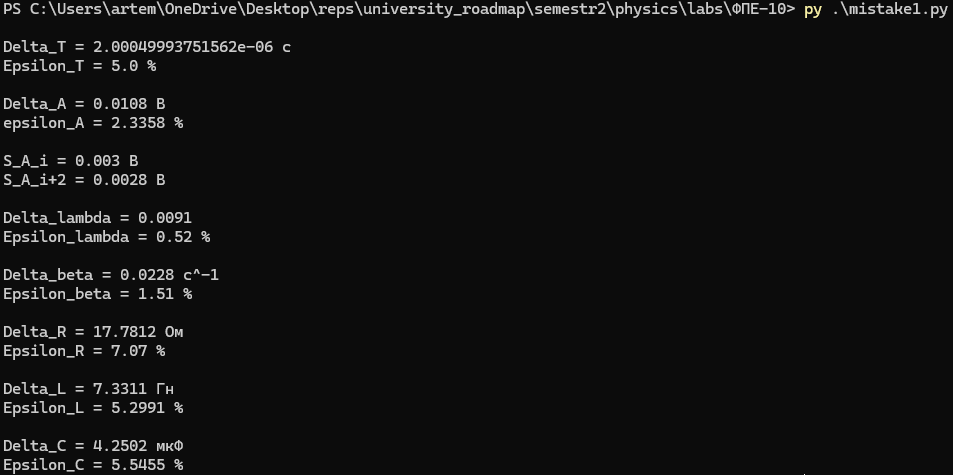
\includegraphics[width=1\textwidth]{mistake1_photo.png}
    \end{figure}

    \vspace{2em} % вручну задаєте відступ

    \textbf{\large Завдання №2:}
    \vspace{1em} % вручну задаєте відступ

    \setlength{\parindent}{1.5em}

    Тут я змінюватиму значення $R_m$, вимірюватиму величини $U_1$ ($I_1$), $U_2$ ($I_2$) та $U_3$ ($I_3$) по горизонталі, що являється зміною напруги між клемами магазину опорів.
    Вертикальні напруги $U_1$, $U_2$ та $U_3$ це напруги між пластинами конденсатора, тобто це ті самі значення напруги, що були в таблиці №1, а це значить, що деякі данні з таблиці №1 я перенесу в таблицю №2 задля
    уникнення повторних вимірювань, що дадуть однаковий результат. Значення сил струмів, отримаю за допомогою 1 закона Ома. За наявних даних, обчислю всі значення таблиці №2 за допомогою Python коду (\hyperlink{listing3}{Лістинг 3.3}).

    \begin{table}[h!]
        \centering
        \renewcommand{\arraystretch}{1.2} % відстань між рядками
        \begin{tabular}{|c|c|c|c|c|c|c|c|c|c|}
            \hline
            $R_m$, Ом & $R_m + r_k$, Ом & $U_1$, В & $U_2$, В & $U_3$, В & $\lambda_U$ & $I_1$, мА & $I_2$, мА & $I_3$, мА & $\lambda_I$ \\ [3pt]
            \hline
            100 & 163 & 5,4547 & 4,5516 & 3,8292 & 0,2359 & 1,8770 & 1,5700 & 1,3100 & 0,2398 \\[3pt]
            200 & 263 & 4,8768 & 3,6485 & 2,7093 & 0,3919 & 1,6380 & 1,2220 & 0,9050 & 0,3953 \\[3pt]
            300 & 363 & 4,3710 & 2,8899 & 1,8785 & 0,5630 & 1,4110 & 0,9437 & 0,6350 & 0,5324 \\[3pt]
            400 & 463 & 3,9014 & 2,2758 & 1,3366 & 0,7141 & 1,2310 & 0,7230 & 0,4303 & 0,7007 \\[3pt]
            500 & 563 & 3,4679 & 1,8423 & 0,9392 & 0,8709 & 1,0590 & 0,5716 & 0,2942 & 0,8539 \\[3pt]
            600 & 663 & 3,0706 & 1,4450 & 0,6864 & 0,9988 & 0,9118 & 0,4272 & 0,1972 & 1,0210 \\[3pt]
            \hline
        \end{tabular}
        \caption{Результати розрахунку $\lambda_U$, $I_1$, $I_2$, $I_3$, $\lambda_I$ коливального контуру.}
    \end{table}

    Значення $\lambda_U$. З огляду на те, що у формулі знаходження логарифмічного декременту згасання оперують лише дві змінні, а у мене їх визначено 3, це значить, що $\lambda_I$ я буду брати як середнє
    арфиметичне цих значень. Згідно результатам виконання програми, обчислені логарифмічний декременти спаданнання для $I$ дорівнює

    \begin{center}
        $\Delta \lambda_I = 0,4242$
    \end{center}

    \setlength{\parindent}{0pt}

    Результат виконання програми з \hyperlink{listing3}{Лістингу 3.3}:

    \begin{figure}[ht]
        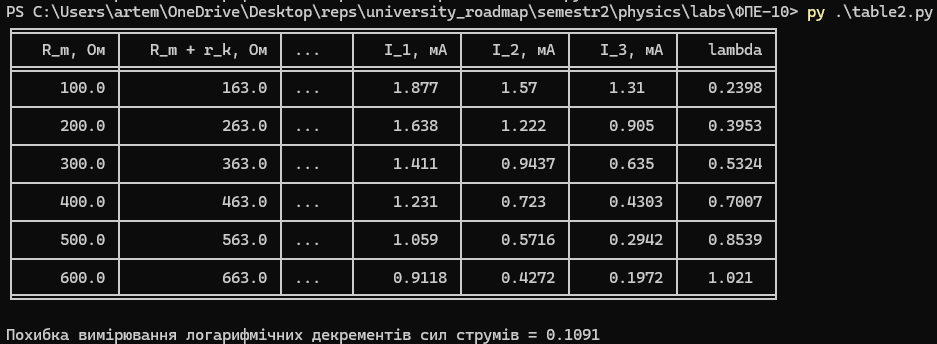
\includegraphics[width=1\textwidth]{table2.png}
    \end{figure}

    Графiк, що демонструє аперiодичне коливання при критичному опорi контуру $R_{cr}$:

    \begin{figure}[ht]
        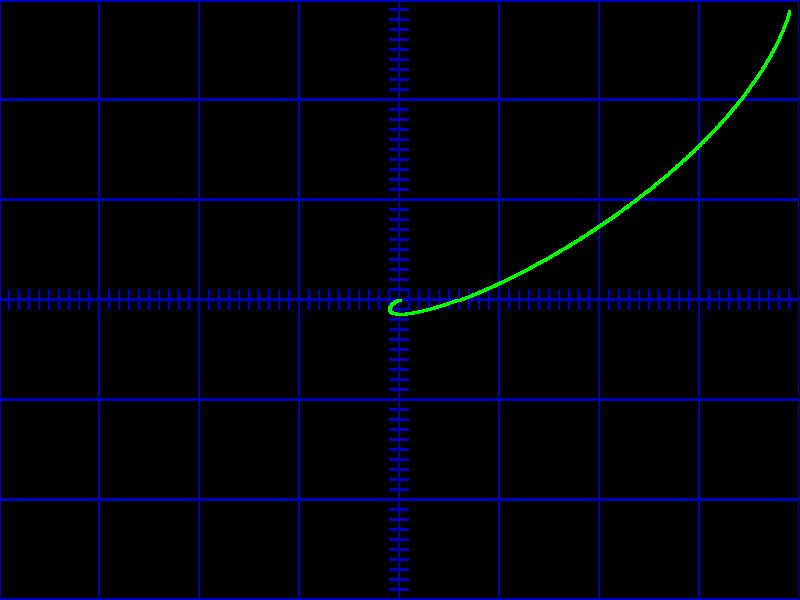
\includegraphics[width=1\textwidth]{aperiodic2.jpg}
    \end{figure}

    \newpage

    Графiк, що демонструє перiодичне незгасне фазове коливання:

    \begin{figure}[ht]
        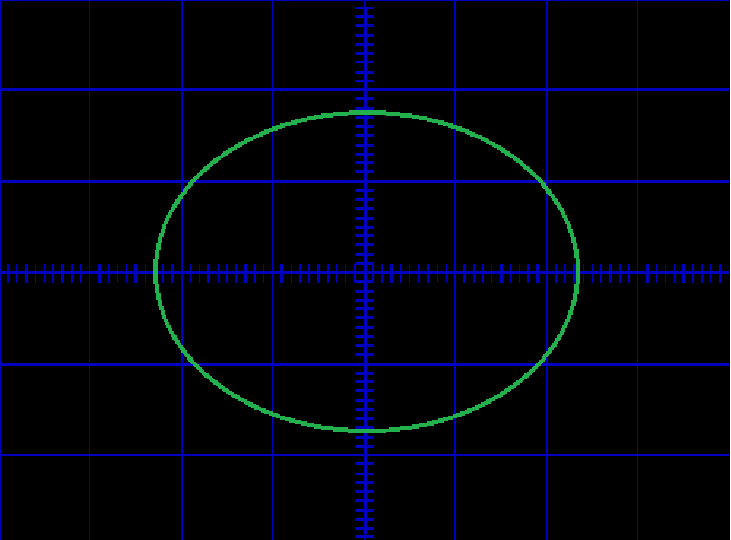
\includegraphics[width=1\textwidth]{YEY1.png}
    \end{figure}

    \newpage

    \textbf{\large Обчислення похибок для завдання №2:}

    \setlength{\parindent}{1.5em}

    \vspace{1em}

    В ході виконання завдання №2, обислювались такі величини: $R_m + r_k$, $U_i$, $I_i$, $\lambda_U$, $\lambda_I$. Для значень
    $R_m + r_k$, $U_i$ та $\lambda_U$ ми попередньо обчислювали. Теоретично обчислені значення: $I_i$ та $\lambda_I$.

    Розглянемо функцію $I_i$, яка обчислювалась за формулою $\displaystyle I_i = \frac{U_i}{R_m}$, відповідно:

    \begin{center}

        $\displaystyle \frac{\partial I_i}{\partial U_i} = \frac{1}{R_m}$; $\displaystyle \frac{\partial I_i}{\partial R_m} = -\frac{U_i}{R_m^2}$;
        $\displaystyle \frac{\partial \ln I_i}{\partial U_i} = \frac{1}{U_i}$; $\displaystyle \frac{\partial \ln I_i}{\partial R_m} = -\frac{1}{R_m}$;

    \end{center}

    \begin{center}

        $\displaystyle \Delta I_i = \sqrt{\left( \frac{S_{U_i}}{\text{⟨}R_m\text{⟩}} \right)^2 + \left( \frac{\text{⟨}U_i\text{⟩}}{\text{⟨}R_m\text{⟩}^2} S_{R_m} \right)^2}$, 
        $\displaystyle \varepsilon_{I_i} = \sqrt{\left( \frac{S_{U_i}}{\text{⟨}U_i\text{⟩}} \right)^2 + \left( \frac{S_{R_m}}{\text{⟨}R_m\text{⟩}} \right)^2} \cdot 100 \%$;
    
    \end{center}

    де $S_{U_i}$ абсолютна похибка вимірювань величин, які ми будемо обчислювати так само, як і обчислювали похибку для $A_i$ і так само, я знайду $\text{⟨}U_i\text{⟩}$. $\text{⟨}R_m\text{⟩} = 350$ Ом, $S_{R_m} = 17,7812$ Ом.
    Похибка вимірювання горизонтальної напруги на екрані (при ціні поділки $\Delta u = 0,03$ В) осцилографа дорівнює $\Delta u \cdot 0,2 = 0,03 \cdot 0,2 = 0,006$ В.
    За результатами програми з Лiстингу 3.4 $\Delta I \approx 0,87 \cdot 10^{-6}$ А, $\varepsilon_I \approx 5,0803$ \%.

    Функція $\lambda_I$ залежить від 3 змінних: $I_i$, $I_{i+1}$ та $I_{i+2}$ через те, що ми знаходимо середнє арифметичне цих окремих значень.
    Але ми можемо сказати, за попереднім досвідом як ми спростили функцію $\lambda$ до 2 змінних, ця функція також буде залежати від 2 змінних: $I_i$ та $I_{i+1}$, відповідно:

    \begin{center}
        $\displaystyle \lambda_I = \frac{2}{3} \ln \frac{I_i}{I_{i+2}}$,
    \end{center}

    звідси

    \begin{center}
        $\displaystyle \frac{\partial \lambda_I}{\partial I_i} = \frac{2}{3I_i}$; $\displaystyle \frac{\partial \lambda_I}{\partial I_{i+2}} = -\frac{2}{3I_{i+2}}$;
    \end{center}

    \begin{center}
        $\displaystyle \frac{\partial \ln \lambda_I}{\partial I_i} = \frac{1}{\ln \frac{I_i}{I_{i+2}}}$; $\displaystyle \frac{\partial \ln \lambda_I}{\partial I_{i+2}} = -\frac{1}{\ln \frac{I_i}{I_{i+2}}}$;
    \end{center}

    Відповідно, вирази для обчислення похибок для $\lambda_I$:

    \begin{center}
        $\displaystyle \Delta \lambda_I = \sqrt{\left( \frac{2}{3\text{⟨}I_i\text{⟩}} S_{I_i} \right)^2 + \left( \frac{2}{3\text{⟨}I_{i+2}\text{⟩}} S_{I_{i+2}}\right)^2}$,
    \end{center}

    \begin{center}
        $\displaystyle \varepsilon_{\lambda_I} = \sqrt{\left( \frac{S_{I_i}}{\ln \frac{\text{⟨}I_i\text{⟩}}{\text{⟨}I_{i+2}\text{⟩}}}\right)^2 + \left( \frac{S_{I_{i+2}}}{\ln \frac{\text{⟨}I_i\text{⟩}}{\text{⟨}I_{i+2}\text{⟩}}} \right)^2} \cdot 100 \% =
        \frac{\sqrt{S_{I_i}^2 + S_{I_{i+2}}^2}}{\ln \frac{\text{⟨}I_i\text{⟩}}{\text{⟨}I_{i+2}\text{⟩}}} \cdot 100 \% = \frac{\sqrt{S_{I_i}^2 + S_{I_{i+2}}^2}}{\ln \text{⟨}I_i\text{⟩} - \ln \text{⟨}I_{i+2}\text{⟩}} \cdot 100 \%$
    \end{center}

    де $S_{I_i} = S_{I_i}$ --- це середні абсолютні похибки вимірювань сил струмів, які нам видасть програма, а $\text{⟨}I_i\text{⟩}$ та $\text{⟨}I_{i+2}\text{⟩}$ --- середні значення сил струмів, також, видасть програма.
    Відповідно до результатів програми з \hyperlink{listing4}{Лістингу 3.4} $\Delta \lambda_I \approx 0,23 \cdot 10^{-9}$, $\varepsilon_{\lambda_I} \approx 0,34$ \%. Прошу помітити, що цей результат відрізняється від результату обчисленні похибки для $\lambda_I$ за формулою, яку ми обчислили у \hyperlink{listing3}{Лістингу 3.3}.
    Це свідчить у потребі додаткової перевірки точності способу вимірювання як у \hyperlink{listing3}{Лістингу 3.3}, так і у \hyperlink{listing4}{Лістингу 3.4} у вільний час, поза межею цієї лабораторної роботи.

    \newpage

    \setlength{\parindent}{0pt}

    Результат виконання програми з \hyperlink{listing4}{Лістингу 3.4}:

    \begin{figure}[ht]
        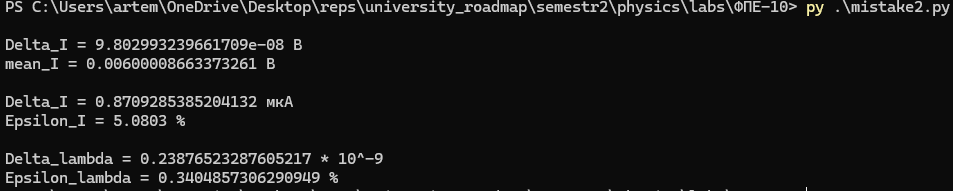
\includegraphics[width=1\textwidth]{mistake2_photo.png}
    \end{figure}

    \vspace{3em}

    \underline{\textbf{\large Висновок:}}

    \vspace{1em}

    У ході лабораторної роботи було точно визначено параметри загасаючих електричних коливань у реальному коливальному контурі.
    Експериментально виміряні значення періоду, логарифмічного декременту, коефіцієнта загасання, індуктивності та
    ємності контуру добре узгоджуються з теоретичними розрахунками. За допомогою аналізу залежності логарифмічного
    декременту від опору було встановлено внутрішній опір котушки, що дозволило коректно розрахувати повний опір контуру
    та критичний опір, при якому спостерігається аперіодичний розряд конденсатора.
    Обчислення похибок показали високу точність вимірювань,
    а використання Python для обробки даних сприяло ефективній оцінці результатів. Значення всіх виміряних похибок:

    \vspace{1em}

    $\Delta R_m \approx 17,5$ Ом, $\varepsilon_{R_m} \approx 5$ \%;

    $\Delta r_k \approx 3,15$ Ом, $\varepsilon_{r_k} \approx 5$ \%;

    $\Delta l \approx 12 \cdot 10^{-6}$ с, $\varepsilon_l \approx 0,3$ \%;

    $\Delta l_1 \approx 12 \cdot 10^{-5}$ с, $\varepsilon_{l_1} \approx 3$ \%;

    $\Delta \nu \approx 0,25$ Гц, $\varepsilon_{\nu} \approx 0,1$ \%;

    $\Delta T \approx 1,69 \cdot 10^{-5}$ с, $\varepsilon_T \approx 4,24$ \%;

    $\Delta A \approx 0,0108$ В, $\varepsilon_A \approx 2,3358$ \%;

    $\Delta \lambda_U \approx 0,0079$ Гн, $\varepsilon_{\lambda_U} \approx 0,52$ \%;

    $\Delta \beta \approx 22,75 \text{ с}^{-1}$, $\varepsilon_{\beta} \approx 4,5$ \%;

    $\Delta R \approx 17,7812$ Ом, $\varepsilon_R \approx 7,07$ \%;

    $\Delta L \approx 0,0079$ Гн, $\varepsilon_L \approx 6,7773$ \%;

    $\Delta C \approx 0,0032$ мкФ, $\varepsilon_C \approx 7,3185$ \%;

    $\Delta R_{cr} \approx 250,3476$ Ом, $\varepsilon_{R_{cr}} \approx 6,0222$ \%.

    $\Delta I \approx 0,87 \cdot 10^{-6}$ А, $\varepsilon_I \approx 5,0803$ \%;

    $\Delta \lambda_I \approx 0,23 \cdot 10^{-9}$, $\varepsilon_{\lambda_I} \approx 0,34$ \%.

    \vspace{3em}

    \newpage

    \begin{center}
        \textbf{\Large Контрольні запитання}
    \end{center}

    \section*{Контрольні питання та відповіді}

    \subsection*{1. Що називають коливальним контуром і як виникають коливання в ньому?}
    \textbf{Відповідь:}  
    Коливальний контур --- це замкнене електричне коло, яке складається з конденсатора ($C$), котушки індуктивності ($L$) та, зазвичай, резистора ($R$). Коливання виникають, коли заряджений конденсатор починає розряджатися через котушку, перетворюючи електричну енергію в магнітну і навпаки. При $R=0$ коливання незгасаючі, а при $R>0$ частина енергії витрачається на нагрівання опору, що призводить до загасання коливань.

    \subsection*{2. Як виводиться рівняння коливного контуру, що містить активний опір $R$?}
    \textbf{Відповідь:}  
    Застосовують другий закон Кірхгофа, записуючи суму напруг по контуру:
    \[
    L\frac{dI}{dt} + RI + \frac{q}{C} = 0,
    \]
    де $q$ --- заряд конденсатора, а струм визначається як $I=-\dfrac{dq}{dt}$.

    \subsection*{3. Який вигляд має розв'язок виведеного рівняння коливного контуру?}
    \textbf{Відповідь:}  
    Розв’язок рівняння для загасаючих коливань має вигляд:
    \[
    U(t)=U_0\, e^{-\beta t}\cos\Bigl(\omega t+\varphi\Bigr),
    \]
    де \(\beta=\dfrac{R}{2L}\) --- коефіцієнт загасання, а \(\omega=\sqrt{\frac{1}{LC}-\Bigl(\frac{R}{2L}\Bigr)^2}\) --- циклічна частота.

    \subsection*{4. За яким законом змінюватиметься напруга на конденсаторі, а також струм, електрична і магнітна енергії в коливному контурі?}
    \textbf{Відповідь:}  
    Напруга та струм у контурі змінюються гармонійно з експоненційним згасанням:
    \[
    \begin{aligned}
    U(t)&=U_0\, e^{-\beta t}\cos(\omega t+\varphi),\\[1ex]
    I(t)&=I_0\, e^{-\beta t}\sin(\omega t+\varphi'),
    \end{aligned}
    \]
    де амплітуди \(U_0\) та \(I_0\) зменшуються за законом \(e^{-\beta t}\).  
    Електрична енергія конденсатора:
    \[
    W_e=\frac{1}{2}C\,U^2(t),
    \]
    а магнітна енергія котушки:
    \[
    W_m=\frac{1}{2}L\,I^2(t).
    \]
    Обидві енергії спадають приблизно як \(e^{-2\beta t}\).

    \subsection*{5. Що таке час загасання і логарифмічний декремент загасання?}
    \textbf{Відповідь:}  
    Час загасання --- це характеристика, що визначає, за який проміжок часу амплітуда коливань зменшується до \(1/e\) від початкової.  
    Логарифмічний декремент загасання визначається як
    \[
    \lambda=\ln\!\left(\frac{A(t)}{A(t+T)}\right),
    \]
    де \(A(t)\) --- амплітуда в момент часу \(t\), \(T\) --- період коливань. При експоненційному загасанні, оскільки \(A(t)=A_0\,e^{-\beta t}\), маємо
    \[
    \lambda=\beta T.
    \]

    \subsection*{6. Як залежить логарифмічний декремент від омічного опору контуру?}
    \textbf{Відповідь:}  
    Оскільки коефіцієнт загасання визначається як \(\beta=\dfrac{R}{2L}\), логарифмічний декремент
    \(\lambda=\beta T\) лінійно зростає із збільшенням опору \(R\) (при постійних \(L\) та \(T\)).

    \subsection*{7. Що таке аперіодичний розряд у контурі і за яких умов він спостерігається?}
    \textbf{Відповідь:}  
    Аперіодичний розряд --- це процес, коли конденсатор розряджається без виникнення осциляцій.  
    Він спостерігається при критичному або надкритичному опорі, тобто коли
    \[
    R \ge R_{\text{кр}} = 2\sqrt{\frac{L}{C}},
    \]
    що не забезпечує умови для осциляцій.

    \subsection*{8. Що таке фазова площина та фазова крива?}
    \textbf{Відповідь:}  
    Фазова площина --- це графік, на якому по одній осі відкладають напругу (наприклад, \(U\)), а по іншій --- струм (наприклад, \(I\)).  
    Фазова крива --- це траєкторія системи в цій площині, яка відображає взаємозв’язок між змінними в процесі коливань.

    \subsection*{9. Яка форма фазової кривої при незагасаючих коливаннях? При загасаючих коливаннях? При аперіодичному процесі?}
    \textbf{Відповідь:}  
    \begin{itemize}
        \item При незгасаючих коливаннях (при \(R=0\)) фазова крива є замкненою (коло або еліпс).
        \item При загасаючих коливаннях (при \(R>0\)) фазова крива є спіральною, що сходиться до центру.
        \item При аперіодичному розряді коливань (при \(R \ge R_{\text{кр}}\)) осциляцій немає, тому фазова крива не формується.
    \end{itemize}

    \subsection*{10. Звідки необхідно подавати напругу на відхиляючі пластини осцилографа для спостереження загасаючих коливань? Фазової кривої?}
    \textbf{Відповідь:}  
    Для спостереження загасаючих коливань напруга подається безпосередньо з конденсатора.  
    Для побудови фазової кривої використовують дві величини:  
    \begin{itemize}
        \item Напруга на конденсаторі (одна вісь, зазвичай вертикальна).
        \item Напруга, пропорційна струму (наприклад, з резистора, що перетинає контур), яка визначає струм (інша вісь, зазвичай горизонтальна).
    \end{itemize}

    \subsection*{11. Поясніть процеси, що проходять у коливному контурі у моменти перетину фазовою кривою осі напруг або осі струмів.}
    \textbf{Відповідь:}  
    Коли фазова крива перетинає осі:
    \begin{itemize}
        \item При перетині осі напруг, струм досягає свого максимуму (адже зміна напруги мінімальна, а швидкість зміни заряду, тобто струм, максимальна).
        \item При перетині осі струм, напруга знаходиться на максимальному або мінімальному значенні.
    \end{itemize}
    Ці моменти відповідають поворотним точкам обміну енергією між конденсатором і котушкою.

    \subsection*{12. За яких умов можна отримати у даному контурі незагасаючі коливання? Які це коливання?}
    \textbf{Відповідь:}  
    Незагасаючі коливання можливі лише за умови відсутності втрат енергії, тобто при $R=0$.  
    Такі коливання називають власними або вільними коливаннями, коли амплітуда залишається сталою, а період визначається лише параметрами контуру:
    \[
    T = 2\pi\sqrt{LC}.
    \]

    \newpage

    \hypertarget{listing1}{}

    \textbf{\large Лістинг 3.1:}

    \vspace{1em}

    \small{

    \begin{verbatim}[breaklines=true]
import numpy as np # Задля обробки масивів даних
from tabulate import tabulate # Задля красивоговиводу таблиці

PERIOD = 0.4e-3 # Обчислений період, сек
R_K = 63.0058 # Обчислений опір котушки індуктивності, Ом

lamda_table = [] # Список логарифмічних декрементів для всіх значень опору R_m
beta_table = [] # Список коефіцієнтів загасання для всіх значень опору R_m, 1/сек
L_table = [] # Список значень індуктивності для всіх значень опору R_m, Гн
C_table = [] # Список значень ємності для всіх значень опору R_m, мкФ
R_table = [] # Список значень загального опору для всіх значень опору R_m, Ом

MAIN_table_data = [] # Загальний список даних для таблиці

# Виміряні значення 3 амплітуд для різних значень опору R_m (змінюється з кожним рядком)
A_data = np.array([

    [5.4547, 4.5516, 3.8292],
    [4.8769, 3.6485, 2.7093],
    [4.3710, 2.8899, 1.8785],
    [3.9014, 2.2758, 1.3366],
    [3.4679, 1.8423, 0.9392],
    [3.0706, 1.4450, 0.6864]

])

# Значення опоів R_m з МО (магазину опорів), Ом
R_m_table = np.array([

    [100],
    [200],
    [300],
    [400],
    [500],
    [600]

])

# Обчислюємо логарифмічні декременти для кожної пари, та потім комбінуємо
їх до одного значення
for row in A_data:

    # Розраховуємо логарифми для всіх пар
    val1 = np.log(row[0] / row[1])
    val2 = np.log(row[0] / row[2])
    val3 = np.log(row[1] / row[2])

    # Середнє арифметичне трьох значень
    mean_val = np.mean([val1, val2, val3])

    # Додаємо в список
    lamda_table.append(mean_val)

# Перетворюємо список на масив (стовпець)
lamda_table = np.array(lamda_table).reshape(-1, 1)

# Обчислюємо коефіцієнт згасання, поділивши кожен елемент масиву
логарифмічних декрементів на період, 1/сек
beta_table = lamda_table / PERIOD

# Обчислюємо загальний опір, додавши до R_m значення r_k, опору котушки індуктивності, Ом
R_table = R_m_table + R_K

# Обчислюємо значення індуктивності для кожного значення опору R_m, Гн
for i, lambda_val in enumerate(lamda_table, start=0):

    R = R_table[i][0]
    L = PERIOD * R / (2*lambda_val)
    L_table.append(L)

# Перетворюємо список на масив (стовпець)
L_table = np.array(L_table).reshape(-1, 1)

# Обчислюємо значення ємності з кожного значення індуктивності L, мкФ
for L_value in L_table:

    C_value = PERIOD**2 / (4 * np.pi**2 * L_value) * 1e6
    C_table.append(C_value)

# Перетворюємо список на масив (стовпець)
C_table = np.array(C_table).reshape(-1, 1)

# Додаємо всі обчислені значення до загального списку даних для таблиці
for R_m_val, lambda_val, beta_val, L_val, C_val, R_val in zip(R_m_table,
lamda_table, beta_table, L_table, C_table, R_table):

    MAIN_table_data.append([R_m_val[0], "...", lambda_val[0], beta_val[0],
L_val[0], C_val[0], R_val[0]])

# Виводимо таблицю
print(tabulate(
    MAIN_table_data,
    headers=["R_m, Ом", "...", "lambda", "beta, c^(-1)", "L, Гн", "C, мкФ", "R, Ом"],
    # назва стовпців
    tablefmt="fancy_grid",    # «красиві» подвійні рамки
    floatfmt=".4"           # науковий формат чисел (або ".6f" для звичайного)
))

L_mean = np.mean(L_table) # Обчислення середнього значення індуктивності L, Гн
C_mean = np.mean(C_table) # Обчислення середнього значення ємності C, мкФ
R_critical = 2 * np.sqrt(L_mean / C_mean * 1e6) - R_K # Обчислення критичного опору R, Ом

# Виводимо середні обчисленні значення індуктивності L, Гн, ємності C, мкФ та
критичного опору R, Ом
print(f"\nСередній значення L = {L_mean:.4} Гн")
print(f"Середній значення C = {C_mean:.4} мкФ")
print(f"Критичний опір R = {round(R_critical, 1)} Ом")
    \end{verbatim}}

    \vspace{3em}

    \hypertarget{listing2}{}

    \textbf{\large Лістинг 3.2:}

    \vspace{1em}

    \small{

    \begin{verbatim}[breaklines=true]
import numpy as np # Задля обробки масивів даних
from tabulate import tabulate # Задля красивоговиводу таблиці
import math

#============================U===============================
Обчислення похибки для U

STUDENT_COEF = 1.73 # Коефіцієнт Стьюдента
T_u = 0.006 # Обчислена похибка вирмірювання горизонтальної напруги на екрані осцилографа

# Масив виміряних горизонатних напруг для всіх значень опору R_m
horizontal_U = np.array([

    [0.1877, 0.1570, 0.1310],
    [0.3275, 0.2443, 0.1810],
    [0.4234, 0.2831, 0.1905],
    [0.4923, 0.2892, 0.1721],
    [0.5295, 0.2858, 0.1471],
    [0.5471, 0.2563, 0.1183]

])

# Масив виміряних опорів R_m
R_m_table = np.array([

    [100],
    [200],
    [300],
    [400],
    [500],
    [600]

])

I_table = horizontal_U / R_m_table # Масив виміряних сил струмів

Delta_I = np.sqrt((I_table * 0.03)**2 + T_u**2) # Масив абсолютних похибок вимірювання
сил струмів

Delta_I_mean = np.mean(Delta_I) # Знаходження середнього значення абсолютної похибки
вимірювання сил струмів

Delta_I1_mean = np.mean(Delta_I[:, 0]) # Знаходження середнього значення абсолютної
похибки вимірювання сил струмів для 1 стовпця
Delta_I3_mean = np.mean(Delta_I[:, 1]) # Знаходження середнього значення абсолютної 
охибки вимірювання сил струмів для 3 стовпця

Delta_I_VALUE = np.sqrt(np.sum((Delta_I - Delta_I_mean)**2) /
(len(Delta_I) * (len(Delta_I) - 1))) *
STUDENT_COEF # Загальне обчислення абсолютної похибки вимірювання сил струмів

# Вивід результатів обрахунків
print(f"\nDelta_I = {Delta_I_VALUE} В")
print(f"mean_I = {Delta_I_mean} В")

#============================I===============================
Обчислення похибки для I

mean_R = 350 # Середнє значення опору R
mean_I = Delta_I_mean # Середнє значення абсолютної похибки вимірювання сил струмів
S_R = 17.7812 # Обчислена абсолютна похибка для R
S_I = Delta_I_VALUE # Обчислена абсолютна похибка для I

# Обчислення абсолютної похибки для I
delta_I = math.sqrt(

    (S_I / mean_R)**2 +
    (S_R * mean_I / mean_R**2)**2

) * 1e6 # для переводу в мкА

# Обчислення відносної похибки для I
Epsilon_I = math.sqrt(

    (S_I / mean_I)**2 +
    (S_R / mean_R)**2

) * 100
Epsilon_I = round(Epsilon_I, 4)

# Вивід результатів обрахунків
print(f"\nDelta_I = {delta_I} мкА")
print(f"Epsilon_I = {Epsilon_I} %")

#============================lambda===============================
Обчислення похибки для lambda

mean_I_i1 = np.mean(Delta_I[:, 0]) # Знаходження середнього
значення абсолютної похибки
вимірювання сил струмів для 1 стовпця
mean_I_i3 = np.mean(Delta_I[:, 2]) # Знаходження середнього
значення абсолютної похибки
вимірювання сил струмів для 3 стовпця

S_I_i1 = np.sqrt(np.sum((Delta_I[:, 0] - Delta_I1_mean)**2) /
(len(Delta_I[:, 0]) * (len(Delta_I[:, 0]) - 1))) # Обчислення загальної
абсолютної похибки вимірювання сил струмів для 1 стовпця

S_I_i3 = np.sqrt(np.sum((Delta_I[:, 2] - Delta_I1_mean)**2) / 
len(Delta_I[:, 2]) * (len(Delta_I[:, 2]) - 1))) # Обчислення загальної
абсолютної похибки вимірювання сил струмів для 3 стовпця

# Обчислення абсолютної похибки для lambda
delta_lambda = math.sqrt(

    ((2 * S_I_i1) / 3 * mean_I_i1)**2 +
    ((2 * S_I_i3) / 3 * mean_I_i3)**2

) * 1e9 # для переводу в нА

# Обчислення відносної похибки для lambda
Epsilon_lambda = math.sqrt(S_I_i1**2 + S_I_i3**2) / (math.log(mean_I_i1)
- math.log(mean_I_i3)) * 100

# Вивід результатів обрахунків
print(f"\nDelta_lambda = {delta_lambda} * 10^{-9}")
print(f"Epsilon_lambda = {Epsilon_lambda} %")
    \end{verbatim}}

    \vspace{3em}

    \hypertarget{listing3}{}

    \textbf{\large Лістинг 3.3:}

    \vspace{1em}

    \small{

    \begin{verbatim}[breaklines=true]

import numpy as np # Задля обробки масивів даних
from tabulate import tabulate # Задля красивоговиводу таблиці

R_K = 63.0058 # Обчислений опір котушки індуктивності, Ом
VERTICAL_PRICE = 2.26 # Вертикальна ціна коливань, В

lambda_table = [] # Список логарифмічних декрементів значень I_1, I_2, I_3,
для всіх значень опору R_m
I_table = [] # Список значень обчислених сил струмів, мА
R_table = [] # Список значень загального опору для всіх значень опору R_m, Ом
delta_I_table = [] # Список значень похибок вимірювання горионтальних
напргуг для кожного зі значень опору R_m (через зміну масштабування)
delta_I_lambda_table = [] # Список значень похибок вимірювання
логарифмічних декрементів для кожного зі значень опору R_m

MAIN_table_data = [] # Загальний список даних для таблиці

# Масив обчислених горизонтальних напруг для кожного
значення опору R_m (змінюється з кожним рядком)
horizontal_U = np.array([

[0.1877, 0.1570, 0.1310],
[0.3275, 0.2443, 0.1810],
[0.4234, 0.2831, 0.1905],
[0.4923, 0.2892, 0.1721],
[0.5295, 0.2858, 0.1471],
[0.5471, 0.2563, 0.1183]

])

# Значення вертикальної напруги для кожного
значення опору R_m (змінюється з кожним рядком)
vertical_U = np.array([

[5.4547, 4.5516, 3.8292],
[4.8769, 3.6485, 2.7093],
[4.3710, 2.8899, 1.8785],
[3.9014, 2.2758, 1.3366],
[3.4679, 1.8423, 0.9392],
[3.0706, 1.4450, 0.6864]

])

# Значення опоів R_m з МО (магазину опорів), Ом
R_m_table = np.array([

[100],
[200],
[300],
[400],
[500],
[600]

])

# Обчислюємо загальний опір, додавши до R_m значення r_k,
опору котушки індуктивності, Ом
R_table = R_m_table + R_K

# Обчислюємо значення сил струмів, поділивши кожен елемен
 масиву горизонтальних напруг на значення відповідного опору R_m, мА
I_table = horizontal_U / R_m_table * 1000

# Обчислюємо логарифмічні декременти для кожної пари,
та потім комбінуємо їх до одного значення
for row in horizontal_U:

# Розраховуємо логарифми для всіх пар
val_12 = np.log(row[0] / row[1])
val_13 = np.log(row[0] / row[2])
val_23 = np.log(row[1] / row[2])

# Середнє арифметичне трьох значень
mean_val = np.mean([val_12, val_13, val_23])

# Додаємо в список
lambda_table.append(mean_val)

# Перетворюємо список на масив (стовпець)
lambda_table = np.array(lambda_table).reshape(-1, 1)

# Додаємо всі обчислені значення до загального списку даних для таблиці
for R_m_val, R_val, I_val, lambda_val in zip(R_m_table, R_table, I_table, lambda_table):

MAIN_table_data.append([R_m_val[0], R_val[0], "...", I_val[0],
I_val[1], I_val[2], lambda_val[0]])

# Список значень похибок вимірювання горионтальних напргуг
(множимо 0.2 до кожного значення за формулою похибки для екранів осцилографа)
delta_I_table = 0.2 * np.array([

[0.06],
[0.11],
[0.17],
[0.22],
[0.26],
[0.31]

])

# Обчислюємо похибки вимірювання логарифмічних
декрементів для кожного зі значень опору R_m
for i, row in enumerate(horizontal_U):

# Знаходимо похибку вимірювання логарифмічних декрементів для всіх 3 пар
delta_lambda_val_12 = np.sqrt(delta_I_table[i][0]**2
/ row[0] + delta_I_table[i][0]**2 / row[1])
delta_lambda_val_13 = np.sqrt(delta_I_table[i][0]**2
/ row[0] + delta_I_table[i][0]**2 / row[2])
delta_lambda_val_23 = np.sqrt(delta_I_table[i][0]**2
/ row[1] + delta_I_table[i][0]**2 / row[2])

# Обчислюємо середнє значення похибки вимірювання логарифмічних декрементів
mean_delta_lambda_val = np.mean([delta_lambda_val_12,
delta_lambda_val_13, delta_lambda_val_23])

# Додаємо в список
delta_I_lambda_table.append(mean_delta_lambda_val)

# Обчислюємо загальне середнє значення похибки вимірювання логарифмічних декрементів
delta_I_lambda_value = np.mean(delta_I_lambda_table)

# Виводимо таблицю
print(tabulate(
MAIN_table_data,
headers=["R_m, Ом", "R_m + r_k, Ом", "...", "I_1, мА",
"I_2, мА", "I_3, мА", "lambda"],        # назва стовпців
tablefmt="fancy_grid",    # «красиві» подвійні рамки
floatfmt=".4"           # науковий формат чисел (або ".6f" для звичайного)
))

# Виводимо значення похибки вимірювання логарифмічних декрементів
print(f"\nПохибка вимірювання логарифмічних
декрементів сил струмів = {round(delta_I_lambda_value, 4)}")

    \end{verbatim}}

    \vspace{3em}

    \hypertarget{listing4}{}

    \textbf{\large Лістинг 3.4:}

    \vspace{1em}

    \small{

    \begin{verbatim}[breaklines=true]
import numpy as np # Задля обробки масивів даних
from tabulate import tabulate # Задля красивоговиводу таблиці
import math

#============================U=============================== Обчислення похибки для U

STUDENT_COEF = 1.73 # Коефіцієнт Стьюдента
T_u = 0.006 # Обчислена похибка вирмірювання горизонтальної напруги на екрані осцилографа

# Масив виміряних горизонатних напруг для всіх значень опору R_m
horizontal_U = np.array([

    [0.1877, 0.1570, 0.1310],
    [0.3275, 0.2443, 0.1810],
    [0.4234, 0.2831, 0.1905],
    [0.4923, 0.2892, 0.1721],
    [0.5295, 0.2858, 0.1471],
    [0.5471, 0.2563, 0.1183]

])

# Масив виміряних опорів R_m
R_m_table = np.array([

    [100],
    [200],
    [300],
    [400],
    [500],
    [600]

])

I_table = horizontal_U / R_m_table # Масив виміряних сил струмів

Delta_I = np.sqrt((I_table * 0.03)**2 + T_u**2)
# Масив абсолютних похибок вимірювання сил струмів

Delta_I_mean = np.mean(Delta_I) # Знаходження середнього значення
абсолютної похибки вимірювання сил струмів

Delta_I1_mean = np.mean(Delta_I[:, 0]) # Знаходження середнього значення
абсолютної похибки вимірювання сил струмів для 1 стовпця
Delta_I3_mean = np.mean(Delta_I[:, 1]) # Знаходження середнього значення
абсолютної похибки вимірювання сил струмів для 3 стовпця

Delta_I_VALUE = np.sqrt(np.sum((Delta_I - Delta_I_mean)**2) /
(len(Delta_I) * (len(Delta_I) - 1))) * STUDENT_COEF 
 Загальне обчислення абсолютної похибки вимірювання сил струмів

# Вивід результатів обрахунків
print(f"\nDelta_I = {Delta_I_VALUE} В")
print(f"mean_I = {Delta_I_mean} В")

#============================I=============================== Обчислення похибки для I

mean_R = 350 # Середнє значення опору R
mean_I = Delta_I_mean # Середнє значення абсолютної похибки вимірювання сил струмів
S_R = 17.7812 # Обчислена абсолютна похибка для R
S_I = Delta_I_VALUE # Обчислена абсолютна похибка для I

# Обчислення абсолютної похибки для I
delta_I = math.sqrt(

    (S_I / mean_R)**2 +
    (S_R * mean_I / mean_R**2)**2

) * 1e6 # для переводу в мкА

# Обчислення відносної похибки для I
Epsilon_I = math.sqrt(

    (S_I / mean_I)**2 +
    (S_R / mean_R)**2

) * 100
Epsilon_I = round(Epsilon_I, 4)

# Вивід результатів обрахунків
print(f"\nDelta_I = {delta_I} мкА")
print(f"Epsilon_I = {Epsilon_I} %")

#============================lambda===============================
Обчислення похибки для lambda

mean_I_i1 = np.mean(Delta_I[:, 0]) # Знаходження середнього значення
абсолютної похибки вимірювання сил струмів для 1 стовпця
mean_I_i3 = np.mean(Delta_I[:, 2]) # Знаходження середнього значення
абсолютної похибки вимірювання сил струмів для 3 стовпця

S_I_i1 = np.sqrt(np.sum((Delta_I[:, 0] - Delta_I1_mean)**2) /
(len(Delta_I[:, 0]) * (len(Delta_I[:, 0]) - 1)))
# Обчислення загальної абсолютної похибки вимірювання сил струмів для 1 стовпця

S_I_i3 = np.sqrt(np.sum((Delta_I[:, 2] - Delta_I1_mean)**2) /
(len(Delta_I[:, 2]) * (len(Delta_I[:, 2]) - 1)))
# Обчислення загальної абсолютної похибки вимірювання сил струмів для 3 стовпця

# Обчислення абсолютної похибки для lambda
delta_lambda = math.sqrt(

    ((2 * S_I_i1) / 3 * mean_I_i1)**2 +
    ((2 * S_I_i3) / 3 * mean_I_i3)**2

) * 1e9 # для переводу в нА

# Обчислення відносної похибки для lambda
Epsilon_lambda = math.sqrt(S_I_i1**2 + S_I_i3**2)
/ (math.log(mean_I_i1) - math.log(mean_I_i3)) * 100

# Вивід результатів обрахунків
print(f"\nDelta_lambda = {delta_lambda} * 10^{-9}")
print(f"Epsilon_lambda = {Epsilon_lambda} %")
    \end{verbatim}
    }

\end{document}